% Copyright 2007 by Till Tantau
%
% This file may be distributed and/or modified
%
% 1. under the LaTeX Project Public License and/or
% 2. under the GNU Public License.
%
% See the file doc/licenses/LICENSE for more details.



\documentclass{beamer}

%
% DO NOT USE THIS FILE AS A TEMPLATE FOR YOUR OWN TALKS�!!
%
% Use a file in the directory solutions instead.
% They are much better suited.
%


% Setup appearance:

\usetheme{Darmstadt}
% \usetheme{default}
% \usetheme{Antibes}
\usefonttheme[onlylarge]{structurebold}
\setbeamerfont*{frametitle}{size=\normalsize,series=\bfseries}
\setbeamertemplate{navigation symbols}{}


% Standard packages

\usepackage[english]{babel}
\usepackage[latin1]{inputenc}
\usepackage{times}
\usepackage[T1]{fontenc}
\usepackage{verbatim}
\usepackage{multirow}
\usepackage{lipsum}
\usepackage{verbatim}


% Setup TikZ

\usepackage{tikz}
\usetikzlibrary{arrows}
\tikzstyle{block}=[draw opacity=0.7,line width=1.4cm]


% Author, Title, etc.

\title[MASON and ECJ integration]{Integrating MASON and ECJ}
\logo{%
    \includegraphics[width=1cm,height=1cm,keepaspectratio]{gmu-logo-1c}~%
    \includegraphics[width=1cm,height=1cm,keepaspectratio]{nsf-logo}%    
}

\author[Khaled]{Khaled Ahsan}

%\begin{comment}
\institute[GMU]
{
	%Autonomous Robotics Lab\\
	%Department of Computer Science\\
	George Mason University\\
	\texttt{atalukde@gmu.edu}
}
%\end{comment}

\date[\today]
{
	MASON Workshop\\
	\today
}


% The main document

\begin{document}

\begin{frame}
  \titlepage
\end{frame}

%\begin{frame}{Outline}
%  \tableofcontents
%\end{frame}


\section{Preliminaries}
	\subsection{MASON and ECJ}
	\begin{frame}
		\frametitle{MASON and ECJ}
		\begin{columns}[c]
                	\column{2.5in}  % slides are 3in high by 5in wide                    
				\begin{itemize}
				\setlength{\itemsep}{1in}
					\item MASON: A fast discrete-event multiagent simulation library
					\item ECJ: Evolutionary computation framework
				\end{itemize}
			\column{2.5in}
				\begin{itemize}
					\item \includegraphics[width=1.5in,height=1.5in,keepaspectratio]{mason.pdf}					
					\item \includegraphics[width=1.5in,height=1.5in,keepaspectratio]{ecj.pdf}
                    		\end{itemize}
		\end{columns}
	\end{frame}
	\subsection{Objectives}
	\begin{frame}
		\frametitle{Objectives}
		\begin{itemize}
			\item \emph{Parameter Identification} -- one of the key problems in computer simulations.
			\item According to MASON manual, \begin{quote}``MASON dovetails nicely with ECJ''\end{quote} -- it was initially designed to be tested with MASON. 
			\item Right parameters are hard to set (considering users' design/experimental goal) 
			\item or, making MASON simulation model more interesting.
			\item ECJ already provides a good collection of stochastic optimization algorithms -- why not using them?
		\end{itemize}
	\end{frame}
%
%
\section{Design Goals}
	\begin{frame}
		\frametitle{Design Goals}
		The basic mechanism of this framework is to encode the MASON model parameters into ECJ \texttt{genomes} and evolve them, the fitness of each ECJ chromosome vector will be assessed by running a MASON simulation with those parameters. 
	\end{frame}
	\begin{frame}
		\frametitle{Design Goals}
		We tried to implement this framework by keeping these 3 key design goals in mind -- 
		\begin{itemize}
			\item Reuse the codes in the existing MASON models extensively.
			\item Minimze the modifications on the existing MASON models.
			\item Apply all necessary MASON model specifications in ECJ parameter files.
			\item In some cases, \emph{Java Reflections} could be a better way to achieve.
		\end{itemize}
	\end{frame}
%
%
\section{Simple GA}
	\subsection{Virus Infection Demo}
		\begin{frame}
			\frametitle{First Example: Simple GA}
			We have tried to optimize the parameters for a \emph{Virus Infection} simulation from MASON. The target parameters were as follows --
			\scriptsize{
			\begin{itemize}
				\item \texttt{DIAMETER}: Diameter of agents' neighbourhood, range $[2, 10]$
				\item \texttt{HEALING\_DISTANE}: Distance of healing influence, range $[5, 40]$
				\item \texttt{INFECTION\_DISTANCE}: Distance of infection influence, range $[5, 40]$
				\item \texttt{NUM\_GOODS}: Initial number of ``healing agents'', range $[4, 8]$
				\item \texttt{NUM\_EVILS}: Initial number of ``infectious agents'', range $[4, 8]$
			\end{itemize}}
		\end{frame}
		\begin{frame}
			\frametitle{GA Result}
				% 2 6 14 7 4
				The optimization goal was to minimize the number of average infected agents. We have used simple real-valued EA. The optimal  evolved parameters are as follows --
				\begin{columns}[c]
					\column{2in}
					\begin{block}{}
					\scriptsize{
					\begin{itemize}
						\item \texttt{DIAMETER}: 2 
						\item \texttt{HEALING\_DITANCE}: 6 
						\item \texttt{INFECTION\_DISTANCE}: 14 
						\item \texttt{NUM\_GOODS}: 7 
						\item \texttt{NUM\_EVILS}: 4
					\end{itemize}}
					\end{block}
					\column{2in}
					\begin{block}{}
						\scriptsize{$\rightarrow$ By keeping the number of healing agents \textbf{high} and infectious agents \textbf{low}, it is possible to achieve minimum infection rate in a relatively \textbf{short} healing and \textbf{long} infection distances. \emph{Is it interesting?}}
				\end{block}
				\end{columns}
		\end{frame}
		\begin{frame}
		\frametitle{First Example: Simple GA}
			The parameters in the virus infection demo code were accessed and manipulated on the ECJ side --
			\begin{block}{}
				\scriptsize{
				\ldots \\
				\texttt{mason-model = \textbf{virus.VirusInfectionDemo}}\\
				\texttt{mason-model.steps = 100}\\
				\texttt{mason-model.generalization-test = 10} \\
				\ldots \\
				\texttt{mason-model.param.0 = \textbf{VirusInfectionDemo.DIAMETER}}\\
				\texttt{pop.subpop.0.species.min-gene.0	= 2}\\
				\texttt{pop.subpop.0.species.max-gene.0 = 10}\\
				\ldots \\
				\texttt{mason-model.param.1 = \textbf{VirusInfectionDemo.HEALING\_DISTANCE}}\\
				\ldots}
			\end{block}
		\end{frame}
		\begin{frame}
		\frametitle{First Example: Simple GA}
			Fine grain generalization may not be achievable, since \emph{Java Reflection}s are decided during the run time -- 
			\begin{block}{}
				\scriptsize{
				\texttt{Field field = theClass.getField(fieldNames[f]);}\\
				\texttt{// this also needs to be generalized, i.e. avoid explicitly naming the 'VirusInfectionDemo'}\\
				\texttt{// and IntegerVectorIndividual}\\
				\texttt{field.setInt((\textbf{VirusInfectionDemo})sim[i], ((IntegerVectorIndividual)ind).genome[f]);}}
			\end{block}
		\end{frame}
%
%
\section{Simple GP}
	\begin{frame}
		\frametitle{Second Example: Simple GP}
		We have tried to optimize the parameters for a \emph{PacMan} simulation from MASON -- 
		\begin{itemize}
			\item This problem was inherently a symbolic regression. 
		\item Evolve the \emph{Pac}'s behaviour using GP.
			\item Reflection like design approach was not suitable in this case.
		\end{itemize}
	\end{frame}
	\begin{frame}	
		\frametitle{Second Example: Simple GP}
		A Live Demo? Not done yet. :-(
	\end{frame}
%
%
\section{Multiobjective EA}
	\begin{frame}
		\frametitle{Large Scale MASON Model Optimization with Distributed MOEA}
		In this example, we have tried to optimize a specialized MASON model for social simulation called \emph{RebeLand}. 
		\begin{itemize}
			\item \emph{RebeLand} is an extensive model for simulating a ``government''.
			\item The goal of the simulation is to closely observe how a government works, by tweaking different parameters.
		\end{itemize}
	\end{frame}
	\begin{frame}
		\frametitle{Large Scale MASON Model Optimization with Distributed MOEA}
		The goal of this experiment was to simulate \emph{corruption} in a government, we had two objectives to maximize -- 
		\begin{itemize}
			\item The government's corruption index (amount of public spending skimmed without notifying)
			\item Average satisfaction of the populace along the course of time.
		\end{itemize}
		\begin{block}{}
		\scriptsize{The \emph{RebeLand} model provides different agents and agent behaviours to simulate the whole scenario quite realistically -- citizens, police force, army, rebels etc.}
	\end{block}
	\end{frame}
	\begin{frame}
		\frametitle{Large Scale MASON Model Optimization with Distributed MOEA}
		The parameters that we targeted to be tweaked with were as follows -- 
		%\begin{block}{}
			\footnotesize{
			\begin{itemize}				
				\item State's corruption rate
				\item State's tax rate
				\item State's maximum reserve rate
				\item State's minimum reserve rate
				\item Minimum benefit share to the populace (i.e. public spending)
				\item Maximum number of police force per capita
				\item Initial reserve army ratio
				\item Standing army size
				\item State's attack frequency (to suppress rebels)
			\end{itemize}}  
		%\end{block}             
	\end{frame}
	\begin{frame}
		\frametitle{Large Scale MASON Model Optimization with Distributed MOEA}	
		The experiment was done using ECJ's distributed evolution mechanism and run on GMU's Hydra cluster, with these settings --
		\begin{itemize}
			\item Population size 60
			\item 30 nodes, two parallel slaves on each node.
			\item Generation 100.
			\item duration: approx. 1 hour
		\end{itemize} 
	\end{frame}
	\begin{frame}
		\frametitle{Large Scale MASON Model Optimization with Distributed MOEA}	
		and the result that we have found were as follows -- 
		\centering
		\includegraphics[width=4.5in,height=3.5in,keepaspectratio,angle=270]{front.eps}	
	\end{frame}
	\begin{frame}
		\frametitle{Large Scale MASON Model Optimization with Distributed MOEA}
		We have picked a solution from the middle region (show in the previous image) of the front and found these parameters -- 
		\footnotesize{
			\begin{itemize}				
				\item State's corruption rate -- \textbf{86\%} 
				\item State's tax rate -- \textbf{77\%}
				\item State's maximum reserve rate -- 84\%
				\item State's minimum reserve rate -- 77\%
				\item Minimum benefit share to the populace (i.e. public spending) -- 98\%
				\item Maximum number of police force per capita -- \textbf{31\%}
				\item Initial reserve army ratio -- 0.01\%
				\item Standing army size -- 0.06\%
				\item State's attack frequency (to suppress rebels) -- \textbf{78\%}
			\end{itemize}} 
	\end{frame}
	\begin{frame}
		\frametitle{Large Scale MASON Model Optimization with Distributed MOEA}
		\begin{block}{}
		\textbf{Lesson:} It's \emph{fine} to run a \emph{corrupt} government and keep people \emph{happy}, if you have high public spending, \emph{large police force} and very \emph{frequent attack} on rebels.
	\end{block}
	\end{frame}
%
%
\section{Conclusions}                   
	\begin{frame}
		\frametitle{Observation}
		\begin{itemize}
			\item Parameter optimization could be very important for assessing a model's validity, finding more interesting insights.
			\item As ECJ is readily available, we should utilize it.
			\item Need to build a generalized/unified framework to plug ECJ capabilities into MASON models. 
		\end{itemize}
	\end{frame}                     
%
%
\section{Questions?}                   
	\begin{frame}                  
		\frametitle{Questions?}
			Questions?
	\end{frame}                     
%----------------------- end of slide --------------------------------------
	\begin{comment}                 
\section{Introduction}
    \subsection{Why Genetic and Evolutionary Computation ?}
    \begin{frame}
        \frametitle{The motivation}
            \begin{columns}[c]
                \column{3.2in}  % slides are 3in high by 5in wide
                    \begin{itemize}
                        \item<1-> How evolution works ?
                        \item<2-> Is there any way to mimic this process ?
                        \item<3-> Is it possible to design a computer program that can use this idea to find solutions of hard problems by itself ?
                        \item<4-> If the simulation works, then why don't we let the machines evolve themselves ?
                    \end{itemize}
                \column{2in}
                    \begin{itemize}
                        \item<1-> \framebox{\includegraphics[width=1.2in,height=0.4in]{evolution.jpg}}
                        \item<2-> \framebox{\includegraphics[width=1in,height=0.4in]{mimic.jpg}}
                        \item<3-> \framebox{\includegraphics[width=1in,height=0.4in]{ga.jpg}}
                        \item<4-> \framebox{\includegraphics[width=0.7in,height=0.4in]{robots.jpg}}
                    \end{itemize}
                    % e.g. \includegraphics[height=2.65in]{graphic}
            \end{columns}
    \end{frame}

    \subsection{Early History}
    \begin{frame}
        \frametitle{Chronological Development}
            \begin{itemize}
                \item<1-> Computer simulations of evolution started as early as in 1954 with the work of Nils Aall Barricelli.
                \item<2-> Starting in 1957 Australian quantitative geneticist Alex Fraser published a series of papers on simulation of artificial selection of organisms with multiple loci controlling a measurable trait.
                \item<3-> Other noteworthy early pioneers include Richard Friedberg, George Friedman, and Michael Conrad, Fraser, Burnell (1970) and Crosby (1973)
                \item<4-> Lawrence J. Fogel invents Evolutionary Programming (Late 1960 - Early 1970)
                \item<5-> Genetic algorithms in particular became popular through the work of John Holland in the early 1970s, and particularly his book \emph{Adaptation in Natural and Artificial Systems} (1975).
            \end{itemize}
    \end{frame}

    \subsection{Recent Trends}
            \begin{frame}[t]
                \frametitle{Mobile Robotics: Evolving The Instinct of A Robot}
                    \begin{block}{}
                       %\onslide<1->
                       Genetic Algorithms are used to find optimized trajectory of Mobile Robots. Many research institutions and companies are conducting cutting edge research on this topic.
                    \end{block}
                    \begin{columns}[t]
                        %\onslide<2->
                        \column{.5\textwidth}
                            \begin{block}{NASA Mars Rover}
                                \includegraphics[width=2.0in, height=1.2in]{marsrover.jpg}
                            \end{block}
                        %\onslide<3->
                        \column{.5\textwidth}
                            \begin{block}{Khepera Mobile Robot}
                                \includegraphics[width=2.0in, height=1.2in]{khepera.jpeg}
                            \end{block}
                    \end{columns}
            \end{frame}

            \begin{frame}[t]
                \frametitle{Evolvable Hardware: Evolving Machines}
                    \begin{block}{}
                            Evolvable hardware is a reconfigurable electronic circuit, which can be changed by a genetic algorithm. Generally they are implemented on Field Programmable Gate Array(FPGA) or Programmable Logic Device (PLD) board.
                    \end{block}
                    \begin{block}{Basic Idea of EHW}
                                \centering
                                \includegraphics[width=2.0in, height=1.0in]{ehw.jpg}
                    \end{block}
            \end{frame}

            \begin{frame}[t]
                \frametitle{Evolvable Programmable Logic Device (PLD)}
                    \begin{block}{}
                                \centering
                                \includegraphics[width=4.0in, height=2.0in]{cellArray.jpg}
                    \end{block}
            \end{frame}

            \begin{frame}[t]
                \frametitle{Evolving The Neural Network: Evolving The Brain}
                    \begin{block}{}
                            Genetic Algorithms can also be used to evolve a Neural Network's weights or connection topology to adapt its capability in uncertain environments.
                    \end{block}
                    \begin{columns}[t]
                        %\onslide<2->
                        \column{.5\textwidth}
                            \begin{block}{Neural Network}
                                \includegraphics[width=2.0in, height=1.2in]{ann.jpg}
                            \end{block}
                    \end{columns}
            \end{frame}
            \begin{frame}[t]
                \frametitle{Evolving The Neural Network: Evolving The Brain}
                    \begin{block}{}
                        Neural network can be represented as a chromosome that can be evolved to highly sophisticated
                        ones, a simulated evolution that mimics natural evolution of brain in different species on earth.
                    \end{block}
                    \begin{columns}[t]
                        %\onslide<2->
                        \column{.5\textwidth}
                            \begin{block}{Chromosome Representation}
                                \centering
                                \includegraphics[width=2.0in, height=1.2in]{annga.jpg}
                            \end{block}
                    \end{columns}
            \end{frame}

            \begin{frame}[t]
                \frametitle{Scheduling and Timetabling: Industry Applications}
                    \begin{block}{}
                       %\onslide<1->
                       Genetic Algorithms are used to find optimized schedule in job-shop or supply chain management.
                       Many scheduling software packages uses GA for hard problems.
                    \end{block}
                    \begin{columns}[t]
                        %\onslide<2->
                        \column{.5\textwidth}
                            \begin{block}{A DAG representing task sequence}
                                \includegraphics[width=2.0in, height=1.2in]{dag.jpg}
                            \end{block}
                        %\onslide<3->
                        \column{.5\textwidth}
                            \begin{block}{A chromosome of the DAG}
                                \includegraphics[width=2.0in, height=1.2in]{schedule.jpg}
                            \end{block}
                    \end{columns}
            \end{frame}

            \begin{frame}[t]
                \frametitle{Design Optimization: The Invention Program}
                    \begin{block}{}
                        Evolutionary design, as it is known, allows a computer to run through tens of millions of variations on an invention until it hits on the best solution to a problem. As its name suggests, evolutionary design borrows its ideas from biology. It takes a basic blueprint and mutates it in a bid to improve it without human input. As in biology, most mutations are worse than the original. But a few are better, and these are used to create the next generation. ... What has changed, in this as in so much else, is the availability and cheapness of computing power. According to John Koza of Stanford University, who is one of the pioneers of the field, evolutionary designs that would have taken many months to run on PCs are now feasible in days. His team at Stanford developed a Wi-Fi antenna for a client.... [Ref. Economist.com (October 3, 2007)]
                    \end{block}
            \end{frame}
            \begin{frame}[t]
                \frametitle{The ST5 high gain antenna developed by NASA}
                    \begin{block}{}
                       %\onslide<1->
                       The Space Technology 5 Project (ST5) is one of NASA's New Millennium Program missions that will launch multiple miniature spacecraft to test innovative concepts and technologies in the harsh environment of space. They are also using GA for designing high gain antennas, which is really hard to design by human in a short time period.
                    \end{block}
                    \begin{columns}[t]
                        %\onslide<2->
                        \column{.5\textwidth}
                            \begin{block}{Antenna on a ST5 satellite}
                                \centering
                                \includegraphics[width=1.25in, height=0.8in]{st5onsat.jpg}
                            \end{block}
                        %\onslide<3->
                        \column{.5\textwidth}
                            \begin{block}{Closeup view}
                                \centering
                                \includegraphics[width=0.7in, height=0.8in]{st5.jpg}
                            \end{block}
                    \end{columns}
            \end{frame}

\section{Working Principles}
    \subsection{How it works ?}
        \begin{frame}[t]
            \frametitle{Basic Idea: The comparison}
                    \begin{columns}[t]
                        %\onslide<2->
                        \column{.5\textwidth}
                            \begin{block}{Nature}
                                \begin{itemize}
                                    \item<1-> Environment \hspace{0.2in} \includegraphics[width=0.5in, height=0.2in]{environment.jpg}\\
                                    \item<2-> Organisms \hspace{0.31in} \includegraphics[width=0.2in, height=0.2in]{organism.jpg}\\
                                    \item<3-> Chromosome \hspace{0.13in} \includegraphics[width=0.4in, height=0.4in]{chromosome.jpg} \\defines an \\organism\\
                                    \item<4-> Gene \hspace{0.66in} \includegraphics[width=0.4in, height=0.4in]{gene.jpg}\\
                                \end{itemize}
                            \end{block}
                        \column{.5\textwidth}
                            \begin{block}{Genetic Algorithm}
                                \begin{itemize}
                                    \item<1-> Problem \hspace{0.34in} \includegraphics[width=0.2in, height=0.2in]{problem.jpg}\\
                                    \item<2-> Solutions \hspace{0.3in} \includegraphics[width=0.5in, height=0.4in]{tsp1.jpg}\\
                                    \item<3-> Chromosome \hspace{0.03in} \includegraphics[width=0.5in, height=0.2in]{gachrom.jpg} \\defines a \\solution\\
                                    \item<4-> Gene \hspace{0.66in} \includegraphics[width=0.4in, height=0.4in]{gagene.jpg}\\
                                \end{itemize}
                            \end{block}
                    \end{columns}
        \end{frame}

        \begin{frame}[t]
            \frametitle{Nature Vs. Genetic Algorithm}
                    \begin{columns}[t]
                        %\onslide<2->
                        \column{.5\textwidth}
                            \begin{block}{Nature}
                            \footnotesize{
                            \begin{itemize}
                                \item<1-> Problem to solve: Find the fittest organism.\\
                                \item<2-> step 1: Start with a set of organisms.\\
                                \item<3-> step 2: Fittest organisms will survive to multiply, others will die.
                                \item<4-> step 3: Mate them and create offsprings.\\
                                \item<5-> step 4: Mutate some of them.\\
                                \item<6-> step 5: Goto step 2
                            \end{itemize}
                            }
                            \end{block}
                        %\onslide<3->
                        \column{.5\textwidth}
                            \begin{block}{Genetic Algorithm}
                            \footnotesize{
                            \begin{itemize}
                                \item<1-> Problem to solve: Find the best solution.\\
                                \item<2-> step 1: Start with a set of random solutions.\\
                                \item<3-> step 2: Evaluate their fitness, select the good solutions, delete others from memory.\\
                                \item<4-> step 2: Mate them and create offspring solutions.\\
                                \item<5-> step 3: Mutate some of them.\\
                                \item<6-> step 5: Goto step 2
                            \end{itemize}
                            }
                            \end{block}
                    \end{columns}
        \end{frame}


    \subsection{A Simple Example: Traveling Salesman Problem (TSP)}
        \begin{frame}[t]
            \frametitle{TSP: Problem Statement}
                \begin{block}{}
                    \scriptsize{
                    Given a number of cities and the costs of traveling from any city to any other city, what is the least-cost round-trip route that visits each city exactly once and then returns to the starting city?}
                \end{block}
                \begin{block}{}
                    \centering
                    \includegraphics[width=1.9in,height=1.8in]{graph.jpg}
                \end{block}
        \end{frame}
        \begin{frame}[t]
            \frametitle{TSP: Representation}
                \begin{block}{}
                    \centering
                    \includegraphics[width=2in,height=1in]{representation.jpg}
                \end{block}
                \begin{block}{}
                    \footnotesize{
                    \begin{itemize}
                        \item<1-> Each gene represents a node
                        \item<2-> Chromosome represents a tour
                        \item<3-> Chromosome length: Total number of nodes + 1
                    \end{itemize}}
                \end{block}
        \end{frame}
        \begin{frame}[t]
            \frametitle{TSP: Fitness Value}
            \begin{block}{}
                    To calculate the fitness, we have add the every consecutive cost from starting gene to ending gene.
            \end{block}
            \begin{block}{}
                    $fitness = \sum_{i=0}^{n}Cost({Gene}_i,{Gene}_{i+1})$\\
            \end{block}
            \begin{block}{}
                    Here,\\
                    \hspace{0.5in}$n$ = length of the chromosome\\
                    \hspace{0.5in}$Gene_i$ = $i^{th}$ gene (corresponding node on the graph)
            \end{block}
        \end{frame}
        \begin{frame}[t]
            \frametitle{TSP: First Step, Initial Population}
                \begin{block}{}
                    \footnotesize{
                    First we start with a set of randomly created solutions. Here each chromosome is an individual and the whole population has 10 individuals. This population size is remained same throughout the evolution process}
                \end{block}
                \begin{block}{}
                    \centering
                    \includegraphics[width=2in,height=1.8in]{initialpop.jpg}
                \end{block}
        \end{frame}
        \begin{frame}[t]
            \frametitle{TSP: Second Step, Selection}
                \begin{block}{}
                    \footnotesize{
                    At this point, we evaluate the fitness of all existing population and select some of them. When selecting, we will try to pick the fitter solutions more frequently and we remove the unfit solutions from the population. Here increased redness indicates individuals with high fitness value.
                    }
                \end{block}
                \begin{block}{}
                    \centering
                    \includegraphics[width=1.5in,height=1.8in]{select.jpg}
                \end{block}
        \end{frame}
        \begin{frame}[t]
            \frametitle{TSP: Third Step, Crossover}
                \begin{block}
                    \footnotesize{
                    We apply the crossover operation to create offsprings from the survived individuals. There are many ways to do the crossover operation. Here \emph{one-point crossover} is illustrated.}
                \end{block}
                \begin{block}{}
                    \centering
                    \includegraphics[width=2in,height=1.5in]{xover.jpg}
                \end{block}
        \end{frame}
        \begin{frame}[t]
            \frametitle{TSP: Third Step, Mutation}
            \begin{block}{}
                \footnotesize{
                Along with crossover, mutation is also applied to create some new solutions in the population. Mutation facilitates the diversity in overall search process.
                }
            \end{block}
            \begin{block}{}
                \centering
                \includegraphics[width=2in,height=1.5in]{mutation.jpg}
            \end{block}
        \end{frame}
        \begin{frame}[t]
            \frametitle{TSP: When to Finish?}
            \begin{block}{}
                \footnotesize{
                We will continue the whole process until a certain number of generations are passed.
                }
            \end{block}
            \begin{block}{The GA Flow Chart}
                \centering
                \includegraphics[width=2.5in,height=2in]{ga.jpg}
            \end{block}
        \end{frame}

    \subsection{Variants}
        \begin{frame}
            \frametitle{Variants}
            \begin{block}{}
            There are many variants of Genetic Algorithm that use similar kind of strategy to solve problems..
                \footnotesize{
                \begin{itemize}
                    \item Evolution strategy
                    \item Differential Evolution
                    \item Evolutionary Algorithm (Genes are not bits, they are real numbers)
                    \item Genetic Programming (Chromosomes may be tree/graph)
                    \item Particle swarm optimization
                    \item Simulated annealing
                    \item Ant colony optimization
                    \item Artificial immune system
                    \item Co-evolutionary algorithm
                    \item Cultural Algorithm etc
                \end{itemize}
                }
            \end{block}
        \end{frame}

\section{What's Next ?}
    \begin{frame}[t]
        \frametitle{The Future of Genetic and Evolutionary Computation}
        \begin{block}{The GOLEM Project}
            \scriptsize{
                The GOLEM(Genetically Organized Lifelike Electro Mechanics) project was initiated by Cornell University and Brandies University during 1999-2001. The objective of this project was to simulate the process of natural evolution to develop autonomous robots. After the simulation, the supercomputer evolved some primitive machines and they are also made into real life model using automated 3D printer. The real life model was similar in characteristics as the simulated ones.}
        \end{block}
                    \begin{columns}[t]
                        %\onslide<2->
                        \column{.5\textwidth}
                            \begin{block}{Evolution}
                                    \centering
                                    \includegraphics[width=2in, height=1in]{evogolem.jpg}\\
                            \end{block}
                        \column{.5\textwidth}
                            \begin{block}{Simulation}
                                    \centering
                                    \includegraphics[width=2in, height=1in]{golemvirt.jpg}\\
                            \end{block}
                    \end{columns}        
    \end{frame}
    \begin{frame}[t]
        \frametitle{The 3D printed and installed real model}
        \begin{block}{}
            \includegraphics[width=\textwidth,height=2in]{golemreal.jpg}
        \end{block}
    \end{frame}

\section{Conclusion}
    \begin{frame}
        \frametitle{Summary}
            \begin{itemize}
                \item Motivation behind Genetic Algorithm
                \item History
                \item Recent Research
                \item Design principle of Genetic Algorithm
                \item Solving Traveling Salesman Problem using Genetic Algorithm
                \item Variants of Genetic Algorithm
                \item Future of Genetic Algorithm
            \end{itemize}
    \end{frame}

\end{comment}

\begin{comment}
\subsection{The Model and the Problem}

\begin{frame}{What is haplotyping and why is it important?}
  You hopefully know this after the previous three talks\dots
\end{frame}

\begin{frame}[t]{General formalization of haplotyping.}
  \begin{block}{Inputs}
    \begin{itemize}
    \item A \alert{genotype matrix} $G$.
    \item The \alert{rows} of the matrix are \alert{taxa / individuals}.
    \item The \alert{columns} of the matrix are \alert{SNP sites /
        characters}.
    \end{itemize}
  \end{block}
  \begin{block}{Outputs}
    \begin{itemize}
    \item A \alert{haplotype matrix} $H$.
    \item Pairs of rows in $H$ \alert{explain} the rows of $G$.
    \item The haplotypes in $H$ are \alert{biologically plausible}.
    \end{itemize}
  \end{block}
\end{frame}


\begin{frame}[t]{Our formalization of haplotyping.}
  \begin{block}{Inputs}
    \begin{itemize}
    \item A genotype matrix $G$.
    \item The rows of the matrix are individuals / taxa.
    \item The columns of the matrix are SNP sites / characters.
    \item<alert@1->
      The problem is directed: one haplotype is known.
    \item<alert@1->
      The input is biallelic: there are only two homozygous
      states (0 and 1) and one heterozygous state (2).
    \end{itemize}
  \end{block}
  \begin{block}{Outputs}
    \begin{itemize}
    \item A haplotype matrix $H$.
    \item Pairs of rows in $H$ explain the rows of $G$.
    \item<alert@1> The haplotypes in $H$ form a perfect phylogeny.
    \end{itemize}
  \end{block}
\end{frame}


\begin{frame}{We can do perfect phylogeny haplotyping efficiently, but
    \dots}
  \begin{enumerate}
  \item \alert{Data may be missing.}
    \begin{itemize}
    \item This makes the problem NP-complete \dots
    \item \dots even for very restricted cases.
    \end{itemize}
    \textcolor{green!50!black}{Solutions:}
    \begin{itemize}
    \item Additional assumption like the rich data hypothesis.
    \end{itemize}
  \item \alert{No perfect phylogeny is possible.}
    \begin{itemize}
    \item This can be caused by chromosomal crossing-over effects.
    \item This can be caused by incorrect data.
    \item This can be caused by multiple mutations at the same sites.
    \end{itemize}
    \textcolor{green!50!black}{Solutions:}
    \begin{itemize}
    \item Look for phylogenetic networks.
    \item Correct data.
    \item<alert@1->
       Find blocks where a perfect phylogeny is possible.
    \end{itemize}
  \end{enumerate}
\end{frame}


\subsection{The Integrated Approach}

\begin{frame}{How blocks help in perfect phylogeny haplotyping.}
  \begin{enumerate}
  \item Partition the site set into overlapping contiguous blocks.
  \item Compute a perfect phylogeny for each block and combine them.
  \item Use dynamic programming for finding the partition.
  \end{enumerate}

  \begin{tikzpicture}
    \useasboundingbox (0,-1) rectangle (10,2);

    \draw[line width=2mm,dash pattern=on 1mm off 1mm]
      (0,1) -- (9.99,1) node[midway,above] {Genotype matrix}
      (0,0.6666) -- (9.99,0.6666)
      (0,0.3333) -- (9.99,0.3333)
      (0,0) -- (9.99,0) node[midway,below] {\only<1>{no perfect phylogeny}};

    \begin{scope}[xshift=-.5mm]
      \only<2->
      {
        \draw[red,block]            (0,.5)   -- (3,.5)
          node[midway,below] {perfect phylogeny};
      }

      \only<3->
      {
        \draw[green!50!black,block] (2.5,.5)   -- (7,.5)
          node[pos=0.6,below] {perfect phylogeny};
      }

      \only<4->
      {
        \draw[blue,block]           (6.5,.5) -- (10,.5)
          node[pos=0.6,below] {perfect phylogeny};
      }
    \end{scope}
  \end{tikzpicture}
\end{frame}

\begin{frame}{Objective of the integrated approach.}
  \begin{enumerate}
  \item Partition the site set into \alert{noncontiguous} blocks.
  \item Compute a perfect phylogeny for each block and combine them.
  \item<alert@1-> Compute partition while computing perfect
    phylogenies.
  \end{enumerate}

  \begin{tikzpicture}
    \useasboundingbox (0,-1) rectangle (10,2);

    \draw[line width=2mm,dash pattern=on 1mm off 1mm]
      (0,1) -- (9.99,1) node[midway,above] {Genotype matrix}
      (0,0.6666) -- (9.99,0.6666)
      (0,0.3333) -- (9.99,0.3333)
      (0,0) -- (9.99,0) node[midway,below] {\only<1>{no perfect phylogeny}};

    \only<2->
    {
      \begin{scope}[xshift=-0.5mm]
        \draw[red,block] (0,.5)   -- (3,.5)
          node[midway,below] {perfect phylogeny}
                         (8,.5) -- (9,.5);

        \draw[green!50!black,block]
          (3,.5)   -- (6,.5)
            node[pos=0.6,below] {perfect phylogeny}
          (6.4,.5)   -- (8,.5)
          (9,.5) -- (10,.5);

        \draw[blue,block] (6,.5) -- (6.4,.5)
          node[midway,below=5mm] {perfect phylogeny};
      \end{scope}
    }
  \end{tikzpicture}
\end{frame}


\begin{frame}{The formal computational problem.}
  We are interested in the computational complexity of \\
  \alert{the function \alert{$\chi_{\operatorname{PP}}$}}:
  \begin{itemize}
  \item It gets genotype matrices as input.
  \item It maps them to a number $k$.
  \item This number is minimal such that the sites can be
    covered by $k$ sets, each admitting a perfect phylogeny.
    \\
    (We call this a \alert{pp-partition}.)
  \end{itemize}
\end{frame}


\section{Bad News: Hardness Results}

\subsection{Hardness of PP-Partitioning of Haplotype Matrices}

\begin{frame}{Finding pp-partitions of haplotype matrices.}
  We start with a special case:
  \begin{itemize}
  \item The inputs $M$ are \alert{already haplotype matrices}.
  \item The inputs $M$ \alert{do not allow a perfect phylogeny}.
  \item What is $\chi_{\operatorname{PP}}(M)$?
  \end{itemize}
  \begin{example}
    \begin{columns}
      \column{.3\textwidth}
      $M\colon$
      \footnotesize
      \begin{tabular}{cccc}
        0 & 0 & 0 & 1 \\
        0 & 1 & 0 & 0 \\
        1 & 0 & 0 & 0 \\
        0 & 1 & 0 & 0 \\
        1 & 0 & 0 & 0 \\
        0 & 1 & 0 & 1 \\
        1 & 1 & 0 & 0 \\
        0 & 0 & 1 & 0 \\
        1 & 0 & 1 & 0
      \end{tabular}%
      \only<2>
      {%
        
\begin{tikzpicture}
          \useasboundingbox (2.9,0);

          \draw [red, opacity=0.7,line width=1cm] (1.7 ,1.9) -- (1.7 ,-1.7);
          \draw [blue,opacity=0.7,line width=5mm] (0.85,1.9) -- (0.85,-1.7)
                                                  (2.55,1.9) -- (2.55,-1.7);
        \end{tikzpicture}
      }
      \column{.6\textwidth}
      \begin{overprint}
        \onslide<1>
        No perfect phylogeny is possible.

        \onslide<2>
        \textcolor{blue!70!bg}{Perfect phylogeny}

        \textcolor{red!70!bg}{Perfect phylogeny}

        $\chi_{\operatorname{PP}}(M) = 2$.

      \end{overprint}
    \end{columns}
  \end{example}
\end{frame}

\begin{frame}{Bad news about pp-partitions of haplotype matrices.}
  \begin{theorem}
    Finding \alert{optimal pp-partition of haplotype matrices}\\
    is equivalent to finding \alert{optimal graph colorings}.
  \end{theorem}

  \begin{proof}[Proof sketch for first direction]
    \begin{enumerate}
    \item Let $G$ be a graph.
    \item Build a matrix with a column for each vertex of $G$.
    \item For each edge of $G$ add four rows inducing\\the
      submatrix $\left(
        \begin{smallmatrix}
          0 & 0 \\
          0 & 1 \\
          1 & 0 \\
          1 & 1
        \end{smallmatrix}\right)$.
    \item The submatrix enforces that the columns lie in different
      perfect phylogenies. \qedhere
    \end{enumerate}
  \end{proof}
\end{frame}

\begin{frame}{Implications for pp-partitions of haplotype matrices.}
  \begin{corollary}
    If $\chi_{\operatorname{PP}}(M) = 2$ for a haplotype matrix $M$,
    we can find an optimal pp-partition in polynomial time.
  \end{corollary}

  \begin{corollary}
    Computing $\chi_{\operatorname{PP}}$ for haplotype matrices is
    \begin{itemize}
    \item $\operatorname{NP}$-hard,
    \item not fixed-parameter tractable, unless
      $\operatorname{P}=\operatorname{NP}$,
    \item very hard to approximate.
    \end{itemize}
  \end{corollary}
\end{frame}


\subsection{Hardness of PP-Partitioning of Genotype Matrices}


\begin{frame}{Finding pp-partitions of genotype matrices.}
  Now comes the general case:
  \begin{itemize}
  \item The inputs $M$ are \alert{genotype matrices}.
  \item The inputs $M$ \alert{do not allow a perfect phylogeny}.
  \item What is $\chi_{\operatorname{PP}}(M)$?
  \end{itemize}
  \begin{example}
    \begin{columns}
      \column{.3\textwidth}
      $M\colon$
      \footnotesize
      \begin{tabular}{cccc}
        2 & 2 & 2 & 2 \\
        1 & 0 & 0 & 0 \\
        0 & 0 & 0 & 1 \\
        0 & 0 & 1 & 0 \\
        0 & 2 & 2 & 0 \\
        1 & 1 & 0 & 0
      \end{tabular}%
      \only<2>
      {%
        
\begin{tikzpicture}
          \useasboundingbox (2.9,0);

          \draw [red, opacity=0.7,line width=1cm] (1.7 ,1.3) -- (1.7 ,-1.1);
          \draw [blue,opacity=0.7,line width=5mm] (0.85,1.3) -- (0.85,-1.1)
                                                  (2.55,1.3) -- (2.55,-1.1);
        \end{tikzpicture}
      }
      \column{.6\textwidth}
      \begin{overprint}
        \onslide<1>
        No perfect phylogeny is possible.

        \onslide<2>
        \textcolor{blue!70!bg}{Perfect phylogeny}

        \textcolor{red!70!bg}{Perfect phylogeny}

        $\chi_{\operatorname{PP}}(M) = 2$.

      \end{overprint}
    \end{columns}
  \end{example}
\end{frame}


\begin{frame}{Bad news about pp-partitions of haplotype matrices.}
  \begin{theorem}
    Finding \alert{optimal pp-partition of genotype matrices}
    is at least as hard as finding \alert{optimal colorings of
      3-uniform hypergraphs}.
  \end{theorem}

  \begin{proof}[Proof sketch]
    \begin{enumerate}
    \item Let $G$ be a 3-uniform hypergraph.
    \item Build a matrix with a column for each vertex of $G$.
    \item For each hyperedge of $G$ add four rows inducing\\ the submatrix
      $\left(
        \begin{smallmatrix}
          2 & 2 & 2 \\
          1 & 0 & 0 \\
          0 & 1 & 0 \\
          0 & 0 & 1
        \end{smallmatrix}\right)
      $.
    \item The submatrix enforces that the three columns do not all lie
      in the same perfect phylogeny. \qedhere
    \end{enumerate}
  \end{proof}
\end{frame}

\begin{frame}{Implications for pp-partitions of genotype matrices.}
  \begin{corollary}
    Even if we know $\chi_{\operatorname{PP}}(M) = 2$ for a genotype matrix $M$,\\
    finding a pp-partition of any fixed size is still
    \begin{itemize}
    \item $\operatorname{NP}$-hard,
    \item not fixed-parameter tractable, unless
      $\operatorname{P}=\operatorname{NP}$,
    \item very hard to approximate.
    \end{itemize}
  \end{corollary}
\end{frame}


\section{Good News: Tractability Results}

\subsection{Perfect Path Phylogenies}

\begin{frame}{Automatic optimal pp-partitioning is hopeless, but\dots}
  \begin{itemize}
  \item The hardness results are \alert{worst-case} results for\\
    \alert{highly artificial inputs}.
  \item \alert{Real biological data} might have special properties
    that make the problem \alert{tractable}.
  \item One such property is that perfect phylogenies are often
    perfect \alert{path} phylogenies:

    In HapMap data, in 70\% of the blocks where a perfect phylogeny
    is possible a perfect path phylogeny is also possible.
  \end{itemize}
\end{frame}


\begin{frame}{Example of a perfect path phylogeny.}
  \begin{columns}[t]
    \column{.3\textwidth}
    \begin{exampleblock}{Genotype matrix}
      $G\colon$
      \begin{tabular}{ccc}
        A & B & C \\\hline
        2 & 2 & 2 \\
        0 & 2 & 0 \\
        2 & 0 & 0 \\
        0 & 2 & 2
      \end{tabular}
    \end{exampleblock}

    \column{.3\textwidth}
    \begin{exampleblock}{Haplotype matrix}
      $H\colon$
      \begin{tabular}{ccc}
        A & B & C \\\hline
        1 & 0 & 0 \\
        0 & 1 & 1 \\
        0 & 0 & 0 \\
        0 & 1 & 0 \\
        0 & 0 & 0 \\
        1 & 0 & 0 \\
        0 & 0 & 0 \\
        0 & 1 & 1
      \end{tabular}
    \end{exampleblock}

    \column{.4\textwidth}
    \begin{exampleblock}{Perfect path phylogeny}
      \begin{center}
        \begin{tikzpicture}[auto,thick]
          \tikzstyle{node}=%
          [%
            minimum size=10pt,%
            inner sep=0pt,%
            outer sep=0pt,%
            ball color=example text.fg,%
            circle%
          ]

          \node [node] {} [->]
            child {node [node] {} edge from parent node[swap]{A}}
            child {node [node] {}
              child {node [node] {} edge from parent node{C}}
              edge from parent node{B}
            };
        \end{tikzpicture}
      \end{center}
    \end{exampleblock}
  \end{columns}
\end{frame}


\begin{frame}{The modified formal computational problem.}
  We are interested in the computational complexity of \\
  the function $\chi_{\alert{\operatorname{PPP}}}$:
  \begin{itemize}
  \item It gets genotype matrices as input.
  \item It maps them to a number $k$.
  \item This number is minimal such that the sites can be
    covered by $k$ sets, each admitting a perfect \alert{path} phylogeny.
    \\
    (We call this a ppp-partition.)
  \end{itemize}
\end{frame}



\subsection{Tractability of PPP-Partitioning of Genotype Matrices}

\begin{frame}{Good news about ppp-partitions of genotype matrices.}
  \begin{theorem}
    \alert{Optimal ppp-partitions of genotype matrices} can be
    computed in \alert{polynomial time}.
  \end{theorem}
  \begin{block}{Algorithm}
    \begin{enumerate}
    \item Build the following partial order:
      \begin{itemize}
      \item Can one column be above the other in a phylogeny?
      \item Can the columns be the two children of the root of a
        perfect path phylogeny?
      \end{itemize}
    \item Cover the partial order with as few compatible chain pairs
      as possible.

      For this, a maximal matching in a special graph needs to be
      computed.
    \end{enumerate}
  \end{block}
  \hyperlink{algorithm<1>}{\beamergotobutton{The algorithm in action}}
  \hypertarget{return}{}
\end{frame}

\section*{Summary}

\begin{frame}
  \frametitle<presentation>{Summary}

  \begin{itemize}
  \item
    Finding optimal pp-partitions is \alert{intractable}.
  \item
    It is even intractable to find a pp-partition when \alert{just two
      noncontiguous  blocks are known to suffice}.
  \item
    For perfect \alert{path} phylogenies, optimal partitions can be
    computed \alert{in polynomial time}.
  \end{itemize}
\end{frame}


\appendix

\section*{Appendix}

\begin{frame}[label=algorithm]{The algorithm in action.}{Computation of
    the partial order.}
  \begin{columns}[t]
    \column{.4\textwidth}
    \begin{exampleblock}{Genotype matrix}
      $G\colon$
      \begin{tabular}{ccccc}
        A & B & C & D & E \\\hline
        2 & 2 & 2 & 2 & 2 \\
        0 & 1 & 2 & 1 & 0 \\
        1 & 0 & 0 & 1 & 2 \\
        0 & 2 & 2 & 0 & 0
      \end{tabular}
    \end{exampleblock}
    \column{.6\textwidth}
    \begin{exampleblock}{Partial order}
      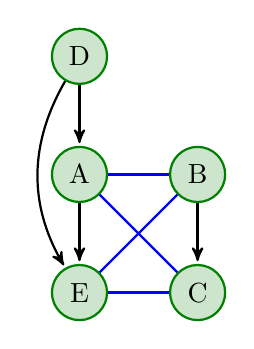
\begin{tikzpicture}[node distance=15mm]
        \tikzstyle{every node}=
        [%
          fill=green!50!black!20,%
          draw=green!50!black,%
          minimum size=7mm,%
          circle,%
          thick%
        ]

        \node (A) {A};
        \node (B) [right of=A] {B};
        \node (C) [below of=B] {C};
        \node (D) [above of=A] {D};
        \node (E) [below of=A] {E};

        \path [thick,shorten >=1pt,-stealth'] (A) edge (E)
                         (B) edge (C)
                         (D) edge (A)
                             edge[bend right] (E);

        \uncover<2>{
        \path [-,blue,thick](A) edge (B)
                                edge (C)
                            (B) edge (E)
                            (C) edge (E);}
      \end{tikzpicture}

      Partial order: \tikz[baseline] \draw[thick,-stealth'] (0pt,.5ex)
      -- (5mm,.5ex);

      \uncover<2>{\textcolor{blue}{Compatible as children of root:
          \tikz[baseline] \draw[thick] (0pt,.5ex) -- (5mm,.5ex);}}
    \end{exampleblock}
  \end{columns}
\end{frame}

\begin{frame}{The algorithm in action.}{The matching in the special graph.}
  \begin{columns}[t]
    \column{.3\textwidth}
    \begin{exampleblock}{Partial order}
      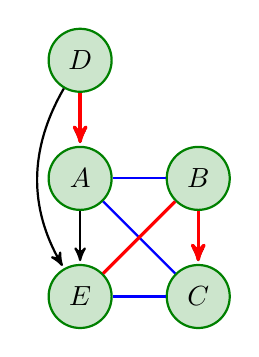
\begin{tikzpicture}[node distance=15mm]
        \tikzstyle{every node}=%
        [%
          fill=green!50!black!20,%
          draw=green!50!black,%
          minimum size=8mm,%
          circle,%
          thick%
        ]

        \node (A)              {$A$};
        \node (B) [right of=A] {$B$};
        \node (C) [below of=B] {$C$};
        \node (D) [above of=A] {$D$};
        \node (E) [below of=A] {$E$};

        \path [thick,shorten >=1pt,-stealth'] (A) edge (E)
                         (B) edge (C)
                         (D) edge (A)
                             edge[bend right] (E);

        \path [-,blue,thick](A) edge (B)
                                edge (C)
                            (B) edge (E)
                            (C) edge (E);

        \only<3->
        {
          \path[very thick,shorten >=1pt,-stealth',red] (D) edge (A) (B) edge (C);
          \path [-,red,very thick](E) edge (B);
        }
      \end{tikzpicture}
    \end{exampleblock}
    \column{.7\textwidth}
    \begin{exampleblock}{Matching graph}
      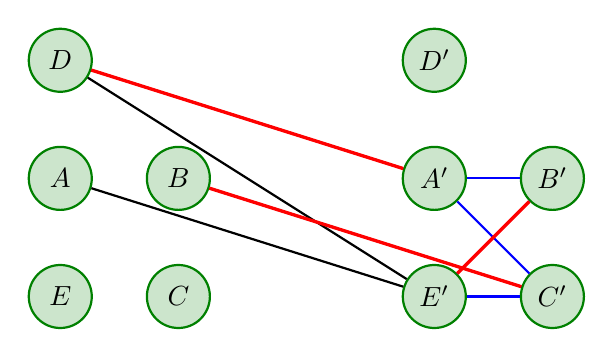
\begin{tikzpicture}[node distance=15mm]
        \tikzstyle{every node}=%
        [%
          fill=green!50!black!20,%
          draw=green!50!black,%
          minimum size=8mm,%
          circle,%
          thick,%
          inner sep=0pt%
        ]

        \node (A)              {$A$};
        \node (B) [right of=A] {$B$};
        \node (C) [below of=B] {$C$};
        \node (D) [above of=A] {$D$};
        \node (E) [below of=A] {$E$};

        \begin{scope}[xshift=4.75cm]
          \node (A')               {$A'$};
          \node (B') [right of=A'] {$B'$};
          \node (C') [below of=B'] {$C'$};
          \node (D') [above of=A'] {$D'$};
          \node (E') [below of=A'] {$E'$};
        \end{scope}

        \path [thick]    (A) edge (E')
                         (B) edge (C')
                         (D) edge (A')
                             edge (E');

        \path [blue,thick](A') edge (B')
                               edge (C')
                          (B') edge (E')
                          (C') edge (E');

        \only<2->
        {
          \path[very thick,red] (D) edge (A')
                           (B) edge (C')
                           (B') edge (E');
        }
      \end{tikzpicture}
    \end{exampleblock}
  \end{columns}

  \medskip
  \uncover<2->{A \alert{maximal matching} in the matching graph
    \uncover<3>{induces\\ \alert{perfect path phylogenies}.}}

  \hfill\hyperlink{return}{\beamerreturnbutton{Return}}
\end{frame}
\end{comment}
\end{document}


